\documentclass[%handout,
	sans,
	12pt,
	%slidescentered,% center text on slide
	%draft,			% compile as draft version
	%notes,			% include notes in slides
	%compress		% compress navigation bar
]{beamer}

\beamertemplatenavigationsymbolsempty

\usetheme{default}
\usecolortheme{orchid}
\setbeamertemplate{frametitle}
{
    \vspace*{1.5em}\insertframetitle\vspace*{-1.5em}
}
\setbeamertemplate{footline}[frame number]

\usepackage[T1]{fontenc}
\usepackage[utf8x]{inputenc}

\usepackage{mathpazo}
\usepackage[british]{babel}
\usepackage{csquotes}

\newcommand{\high}[1]{{\usebeamercolor[fg]{structure} #1}}
\newcommand{\bad}[1]{\textcolor{red}{#1}}
\newcommand{\gray}[1]{\textcolor{darkgray}{#1}}
\newcommand{\black}[1]{\textcolor{black}{#1}}

\usepackage{amsmath,amssymb}
\usepackage{upgreek}
\usepackage{booktabs}
\usepackage{hyperref}
\usepackage{graphicx}
\usepackage{colortbl}
\usepackage{url}
\usepackage{setspace}
\usepackage{wrapfig}
\usepackage{tabularx}
\usepackage{xspace}
\usepackage{mathpartir}

\usepackage{tikz}
\usetikzlibrary{trees, positioning}
\usetikzlibrary{shapes.geometric}

\usepackage{isabelle,isabellesym}
\isabellestyle{it}
\def\isacartoucheopen{}%
\def\isacartoucheclose{}%

\newcommand{\NN}{\mathbb{N}}
\newcommand{\QQ}{\mathbb{Q}}
\newcommand{\RR}{\mathbb{R}}
\newcommand{\CC}{\mathbb{C}}
\renewcommand{\epsilon}{\varepsilon}
\renewcommand{\phi}{\varphi}
\def\braces#1{[#1]}
\newcommand{\wrt}{w.\,r.\,t.\xspace}
\newcommand{\eg}{e.\,g.\xspace}
\newcommand{\ie}{i.\,e.\xspace}
\DeclareMathOperator\caret{\char`\^}

\newcommand{\hastype}{\,:\,}
\newcommand{\cons}{::}
\newcommand{\corrto}{\overset{\scriptscriptstyle\wedge}{=}}
\newcommand{\listapp}{\mathbin{@}}
\newcommand{\listnil}{[\hskip0.3mm]}
\newcommand{\listnth}{\mathbin{!}}
\newcommand{\expectation}{\text{\upshape E}}

\usepackage{manfnt}
\newenvironment{danger}{\medbreak\noindent\hangindent=2pc\hangafter=-2%
  \clubpenalty=10000%
  \hbox to0pt{\hskip-\hangindent\hskip0.25em\raisebox{-0.25em}[0pt][0pt]{\dbend}\hfill}\small\ignorespaces}%
  {\medbreak\par}
  %\raisebox{-1.05em}[0pt][0pt]{\Huge\hskip.15em \stixdanger}

\newcommand{\etAl}{\textit{et al.}\xspace}

%\definecolor{mybg}{rgb}{0.9,0.9,0.9}
\definecolor{mybg}{rgb}{1,1,1}
\setbeamercolor{background canvas}{bg=mybg}

\title{Verification of an Approximation Algorithm for the Metric Travelling Salesperson Problem}
\author{\normalsize Fabian Hellauer}
\institute[]{\footnotesize Technische Universität München}
\date{\footnotesize16 October 2019}

\begin{document}

\maketitle

\begin{frame}
\begin{center}
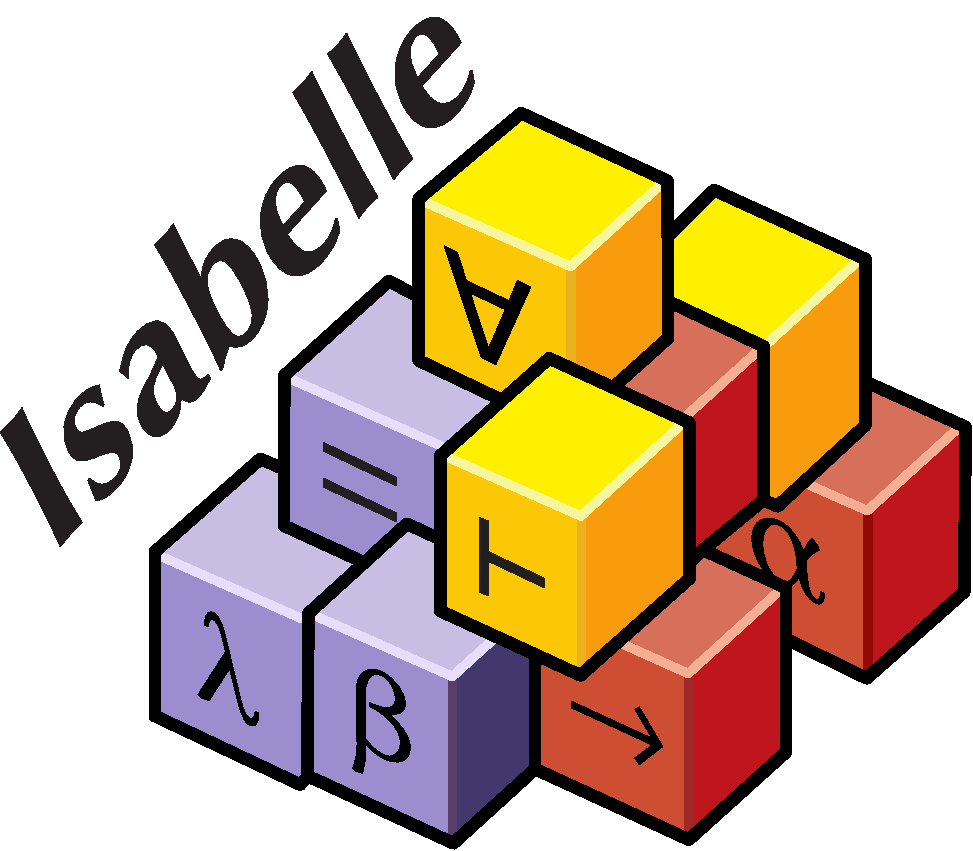
\includegraphics[width=5cm]{isabelle.pdf}
\end{center}
\end{frame}

\newcommand{\pivot}[1]{{\color{red}#1}}
\newcommand{\ltpiv}[1]{{\color{blue}#1}}
\newcommand{\gtpiv}[1]{{\color{olive}#1}}

\section{Verification of Algorithms}
\begin{frame}{Verification of Algorithms}%<very fast>
Reasons:
\begin{itemize}
	\item a basis for reliable software\pause
	\item find mistakes in algorithm explanations\pause
	\item prove that verification of executable programs
	is feasible\ % when using a modern tool like
	\pause when using 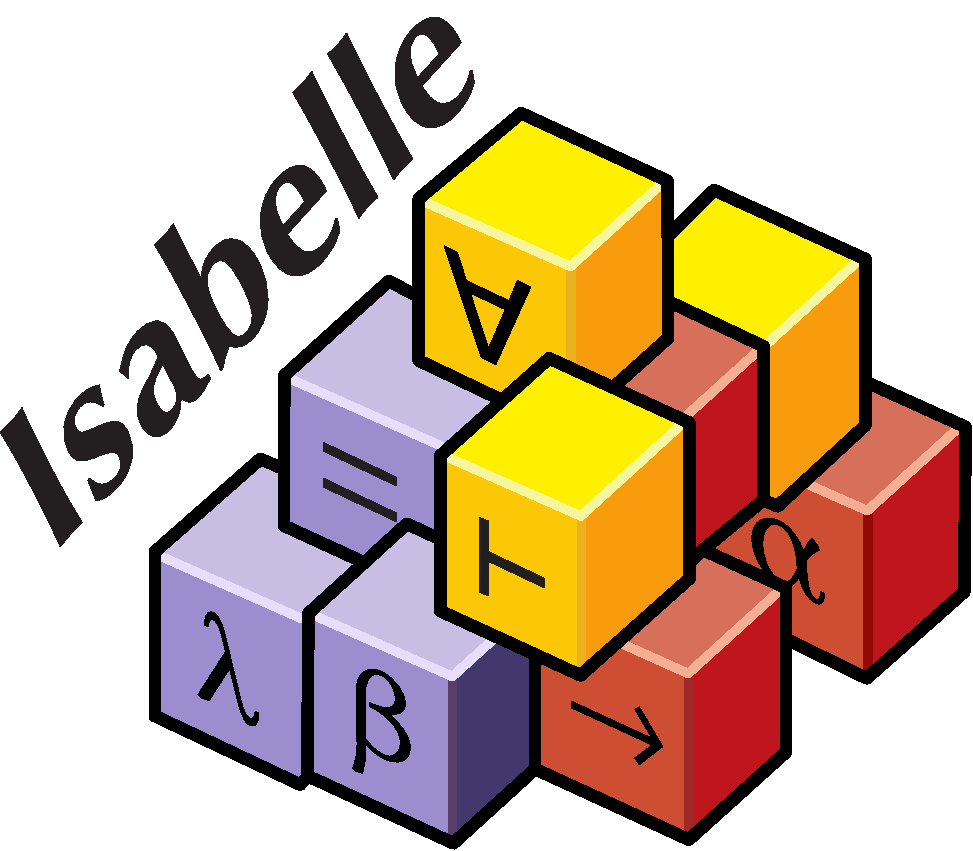
\includegraphics[height=1em]{isabelle.pdf}Isabelle\pause
\end{itemize}
Mathematical results might be a requirement.
%In this case here, from graph theory.
\end{frame}

\section{Metric TSP}
\begin{frame}
	TSP is the problem of finding a tour of minimal cost within a graph.\\\pause
	We consider the special case where the nodes form a \textit{metric space} with their weights.\\\pause
	In particular,\pause
	\begin{itemize}
		\item \textit{weight} is total
		% All TSP cities are connected by an edge, in other words we require the graph to be complete.
		\item $\textit{weight}\ v_1\ v_3\ \leq\ \textit{weight}\ v_1\ v_2\ +\ \textit{weight}\ v_2\ v_3$
		\item $0\ \leq\ \textit{weight}\ v_1\ v_2$\pause
	\end{itemize}
	In such a graph, the cost of a \textit{minimum spanning tree} is a lower bound on the optimal tour cost.
\end{frame}

\section{Approximation Algorithms}
\begin{frame}{Approximation Algorithms}
	What are Approximation Algorithms?\pause%based on (metric) TSP
	\vspace{1em}
	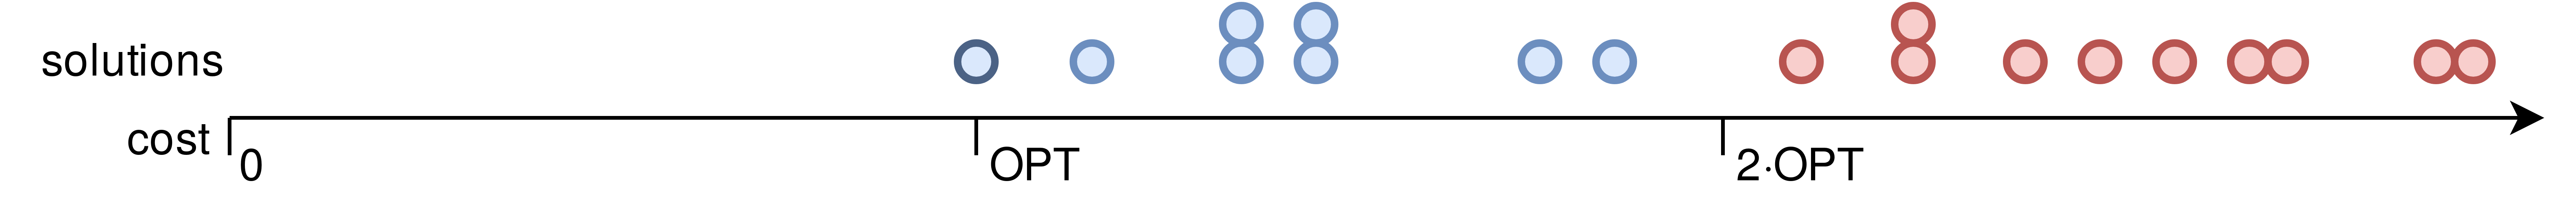
\includegraphics[width=\linewidth]{OPT_line}
	%OPT is the performance of an *actual* algorithm, namely the brute-force algorithm that tries all exponentially many node sequences.
	\vspace{1em}\pause %Since we consider undirected graphs, the reverse of a TSP tour is also a TSP tour (I omitted these duplicates in the graphic)
	
	\high{Good solutions for NP-complete problems in polynomial time!}
\end{frame}

\section{Algorithm Explanation}
\begin{frame}
\begin{center}
	\huge\high{Algorithm Explanation}
\end{center}
\end{frame}

\subsection{Algorithm Overview}
\begin{frame}{Algorithm Overview}
Consider a complete undirected graph$G = (V, E)$ and its minimum spanning tree $T$.\pause%or rather: let one of its minimum spanning trees be $T$

We are going to
\begin{enumerate}
	\item find such a $T$\pause
	\item generate a TSP tour using $T$'s edges
\end{enumerate}% and we are going to argue that T has cost less than an optimal TSP tour
\end{frame}

\subsection{MST vs.\ TSP tour}
\begin{frame}{MST vs.\ TSP tour}
\begin{center}
	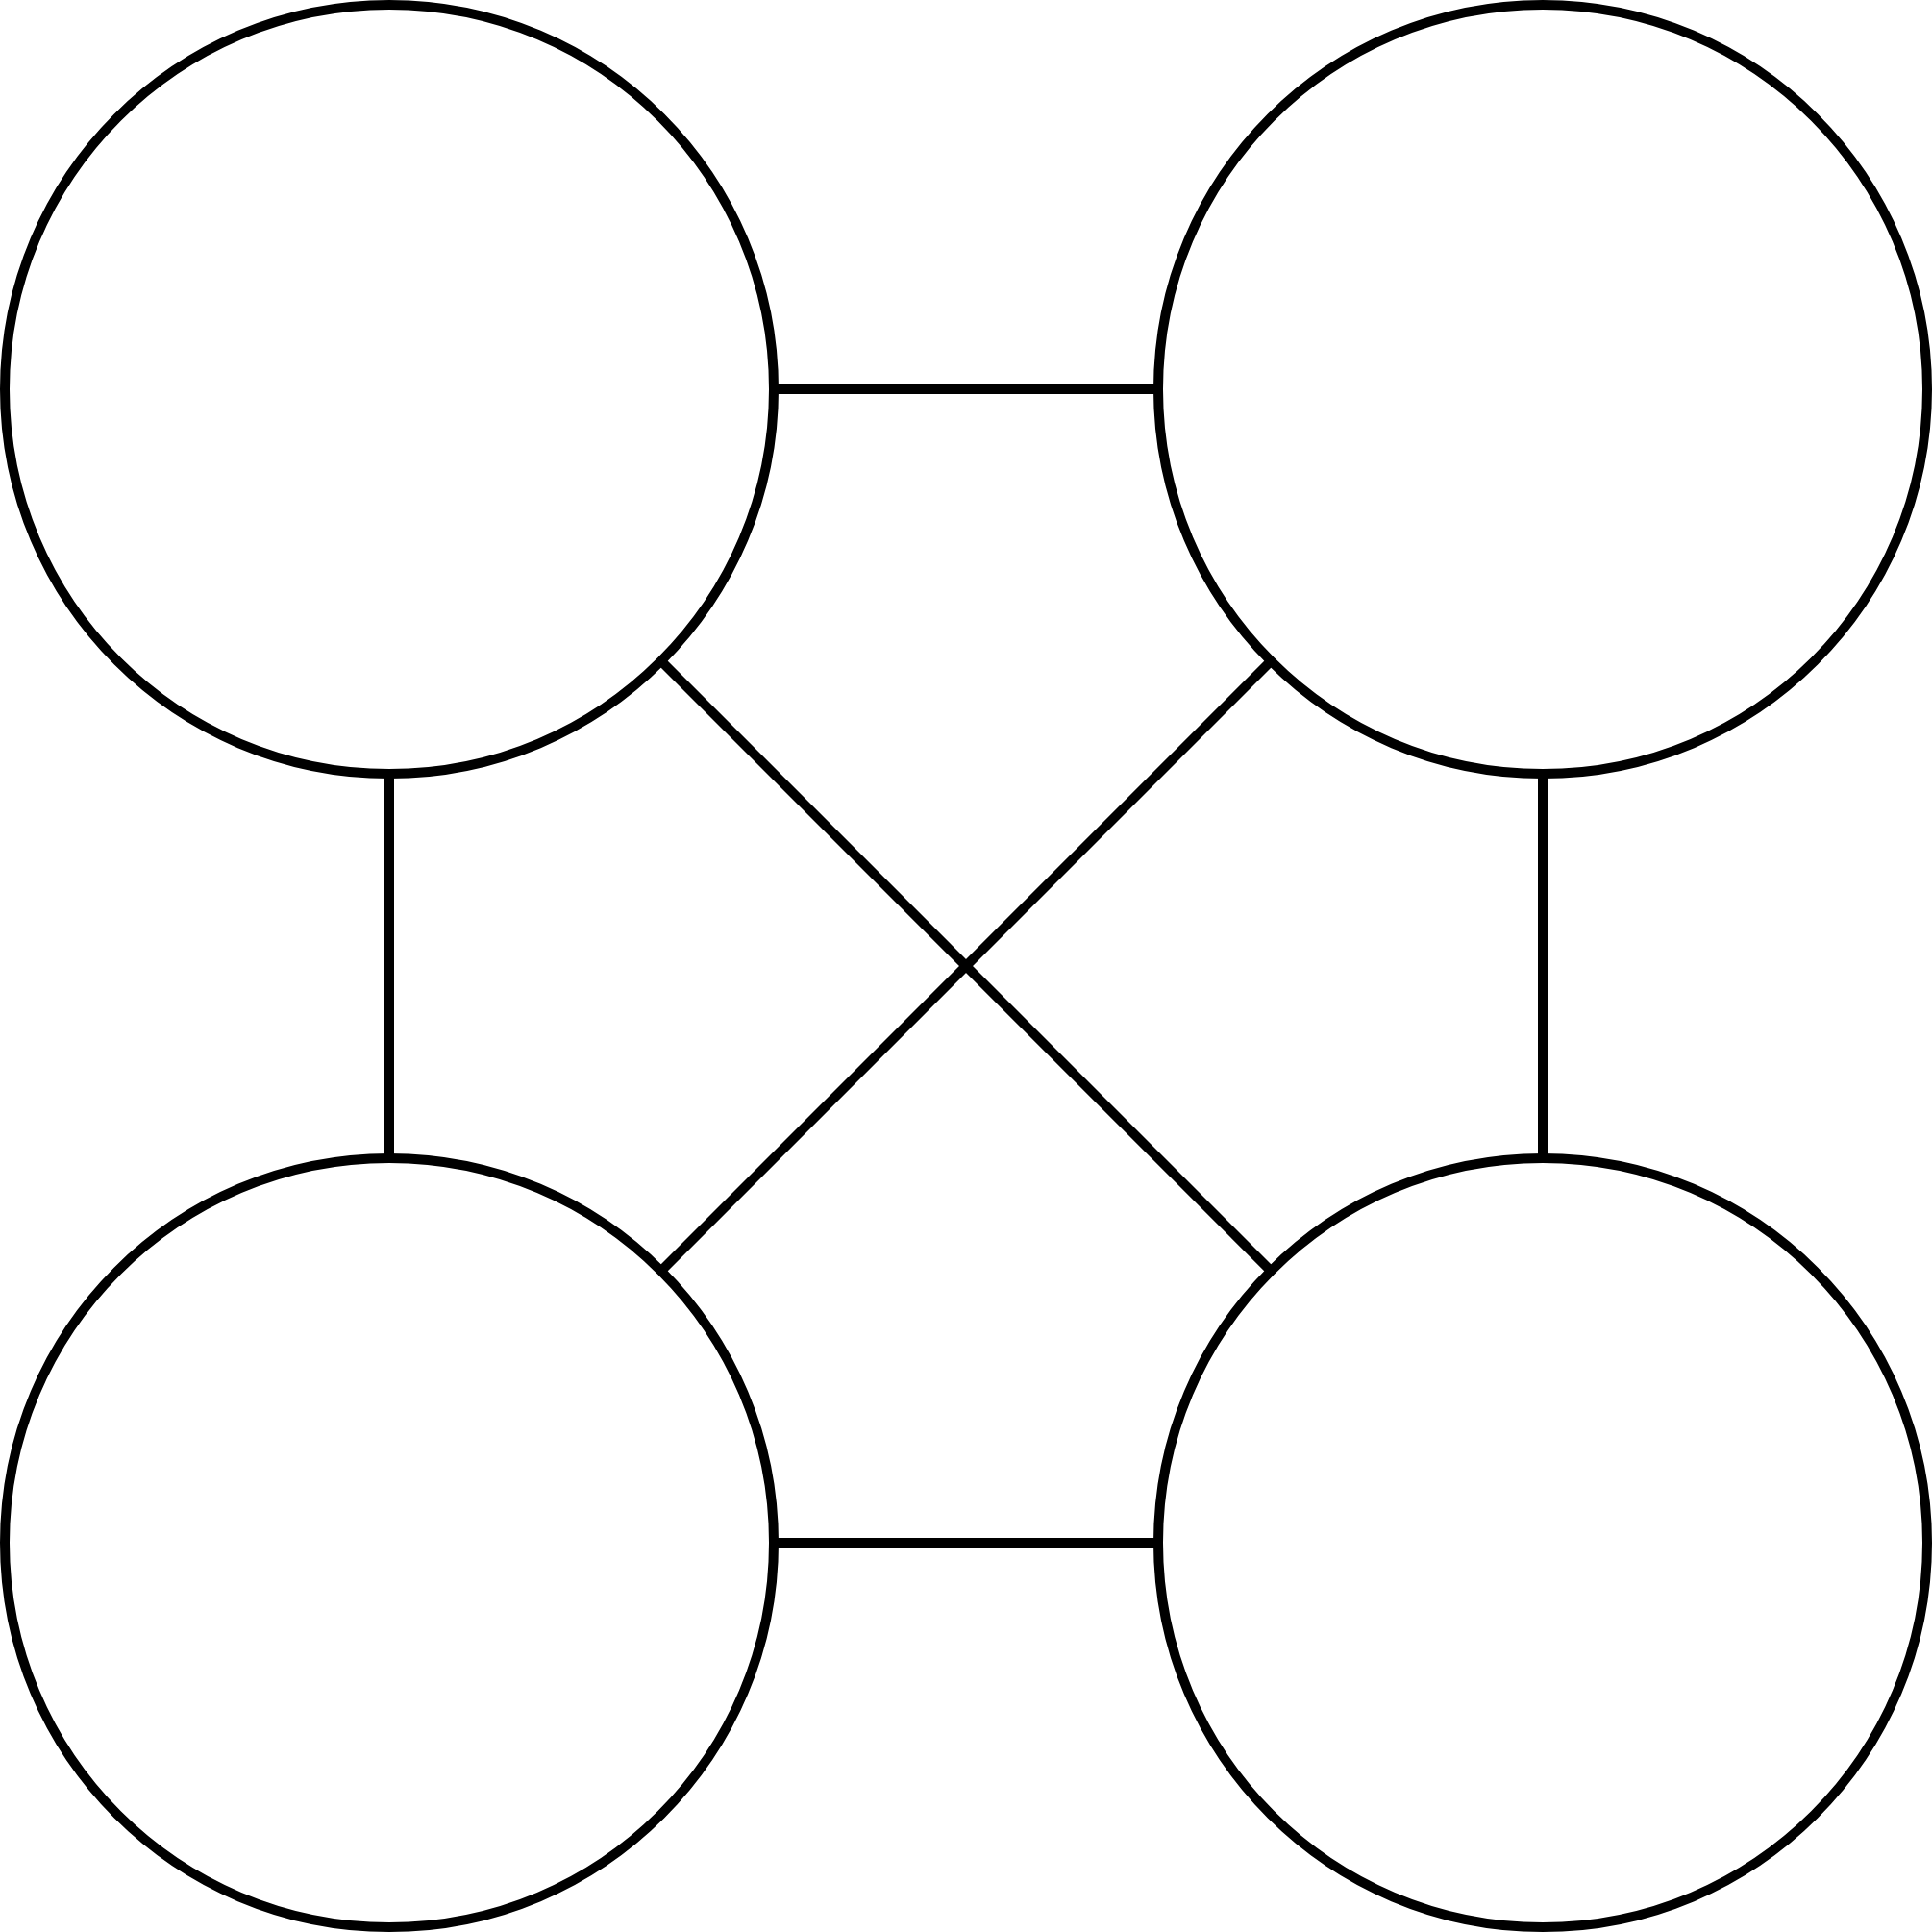
\includegraphics[height=2cm]{complete0.png}
\end{center}
\end{frame}

\subsection{MST vs.\ TSP tour}
\begin{frame}{MST vs.\ TSP tour}
\begin{center}
	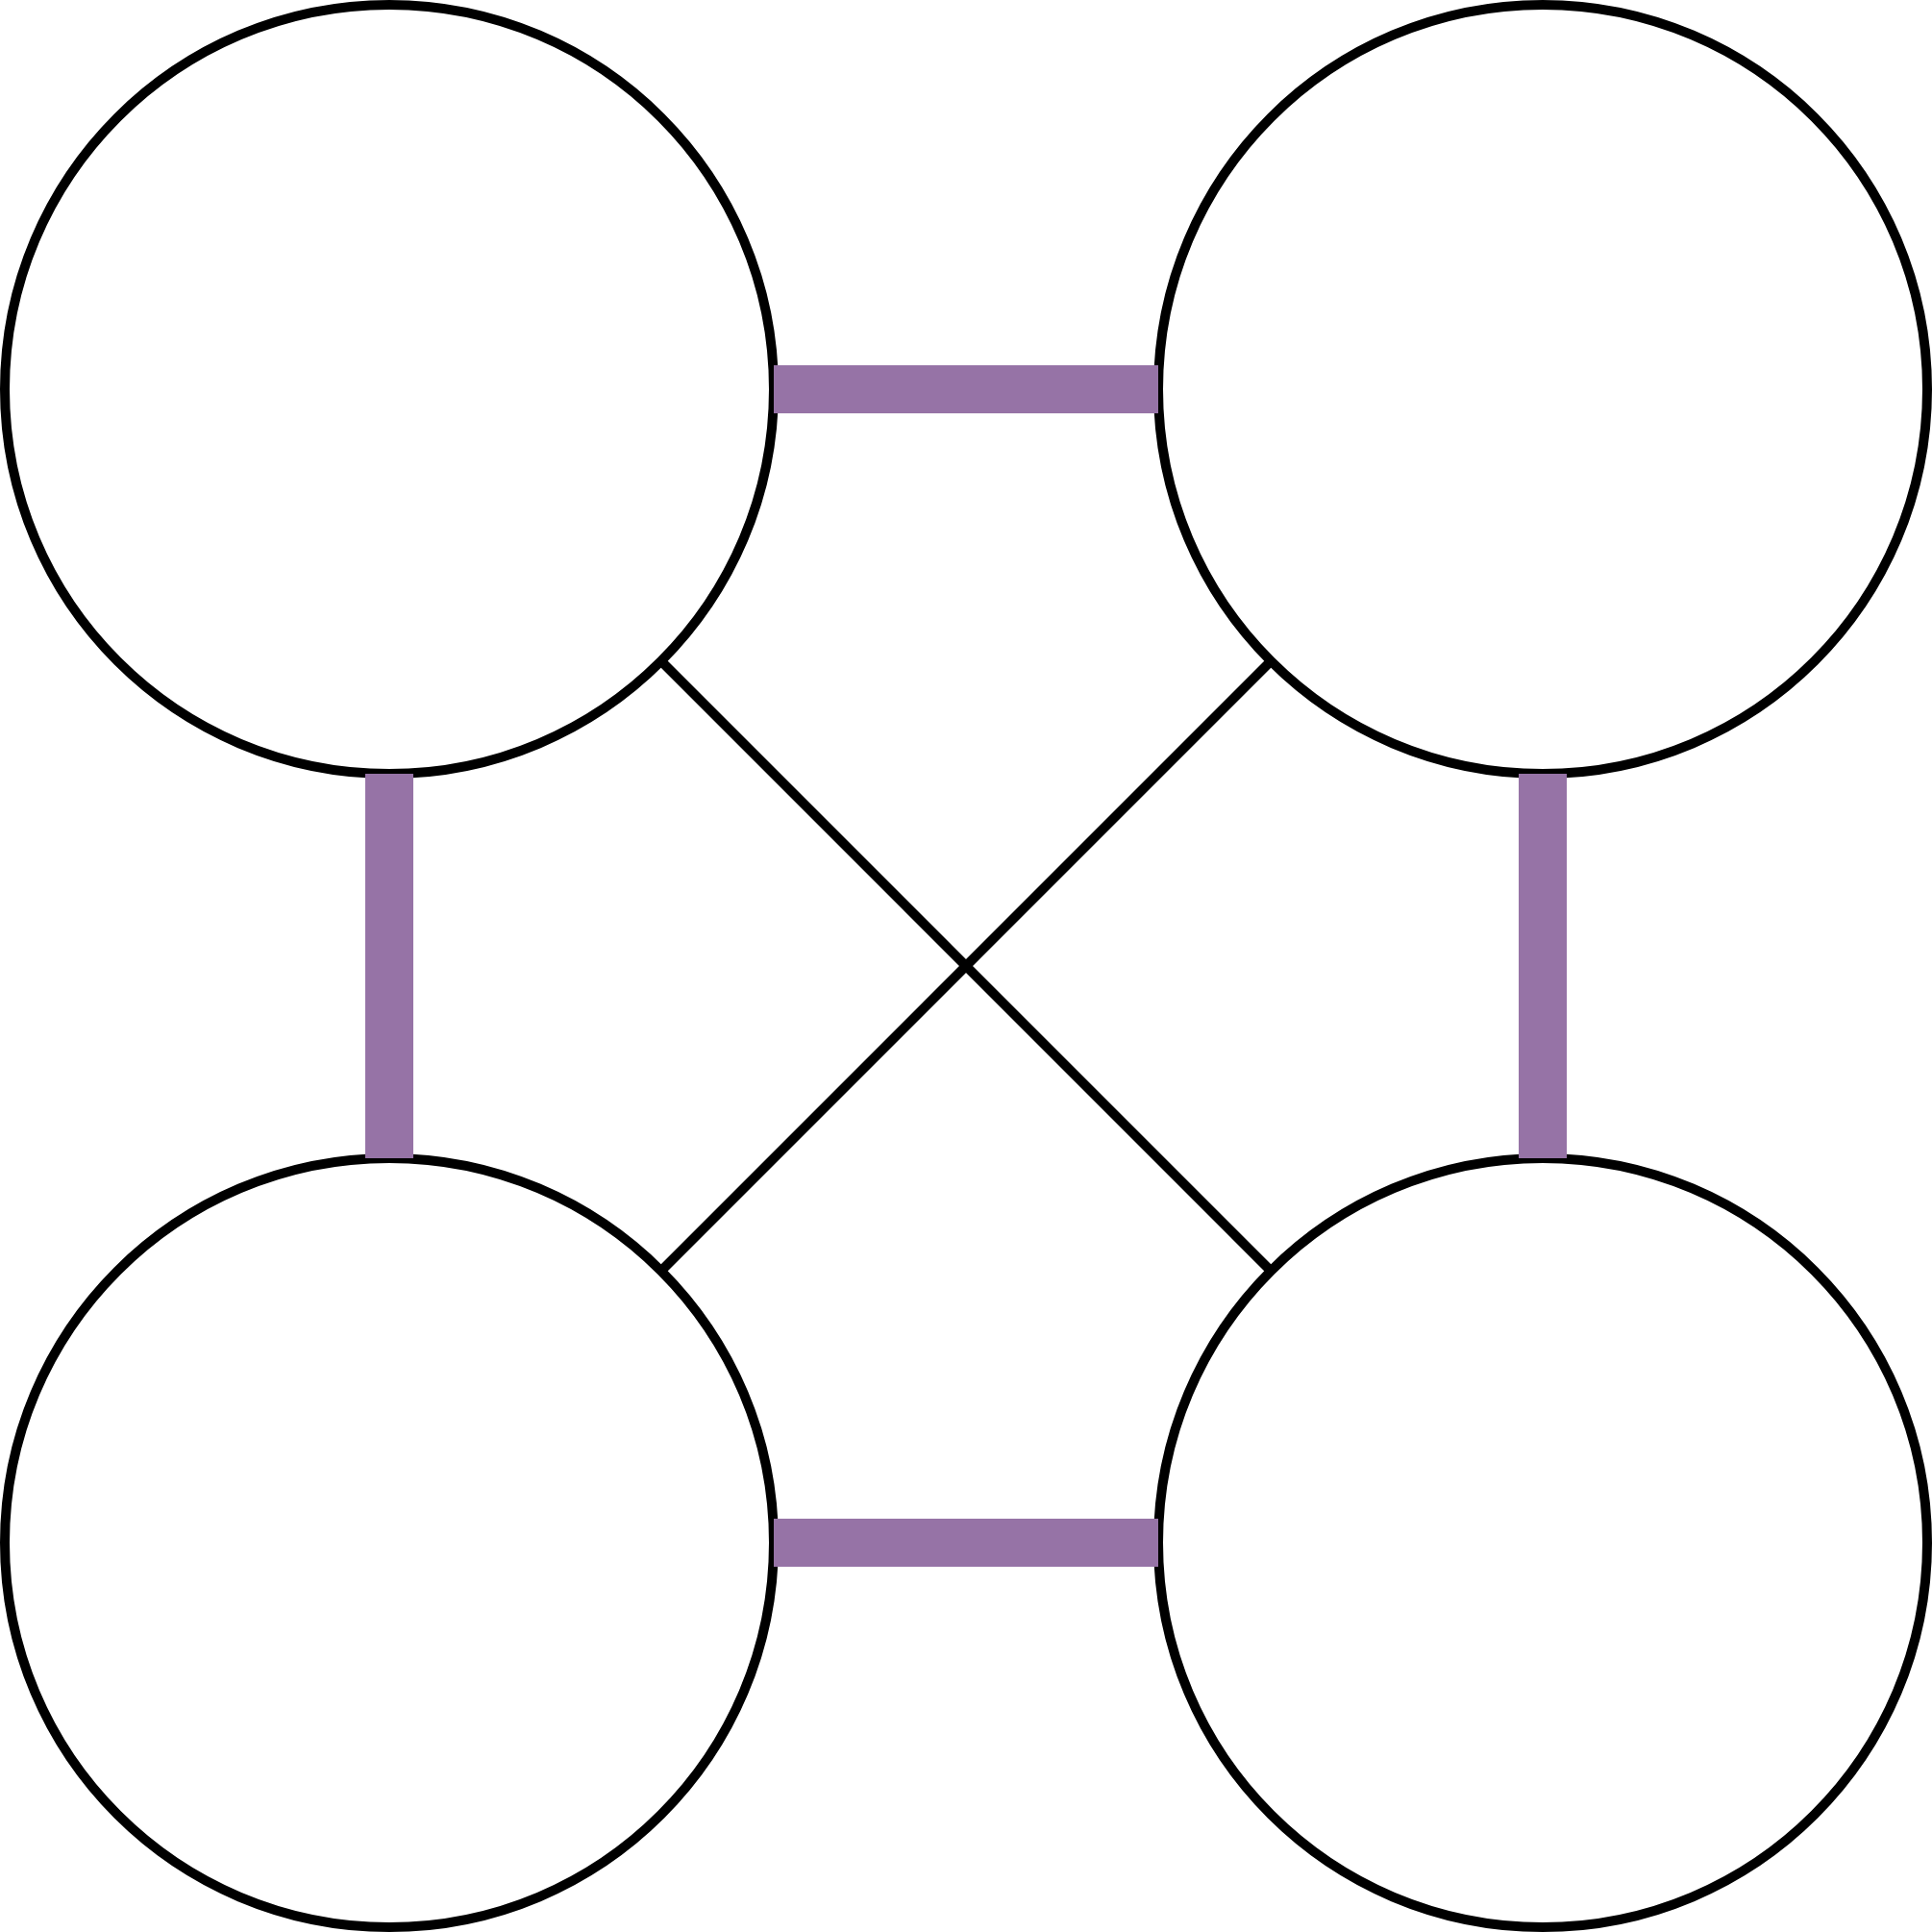
\includegraphics[height=2cm]{complete1.png}
\end{center}
\end{frame}

\subsection{MST vs.\ TSP tour}
\begin{frame}{MST vs.\ TSP tour}
\begin{center}
	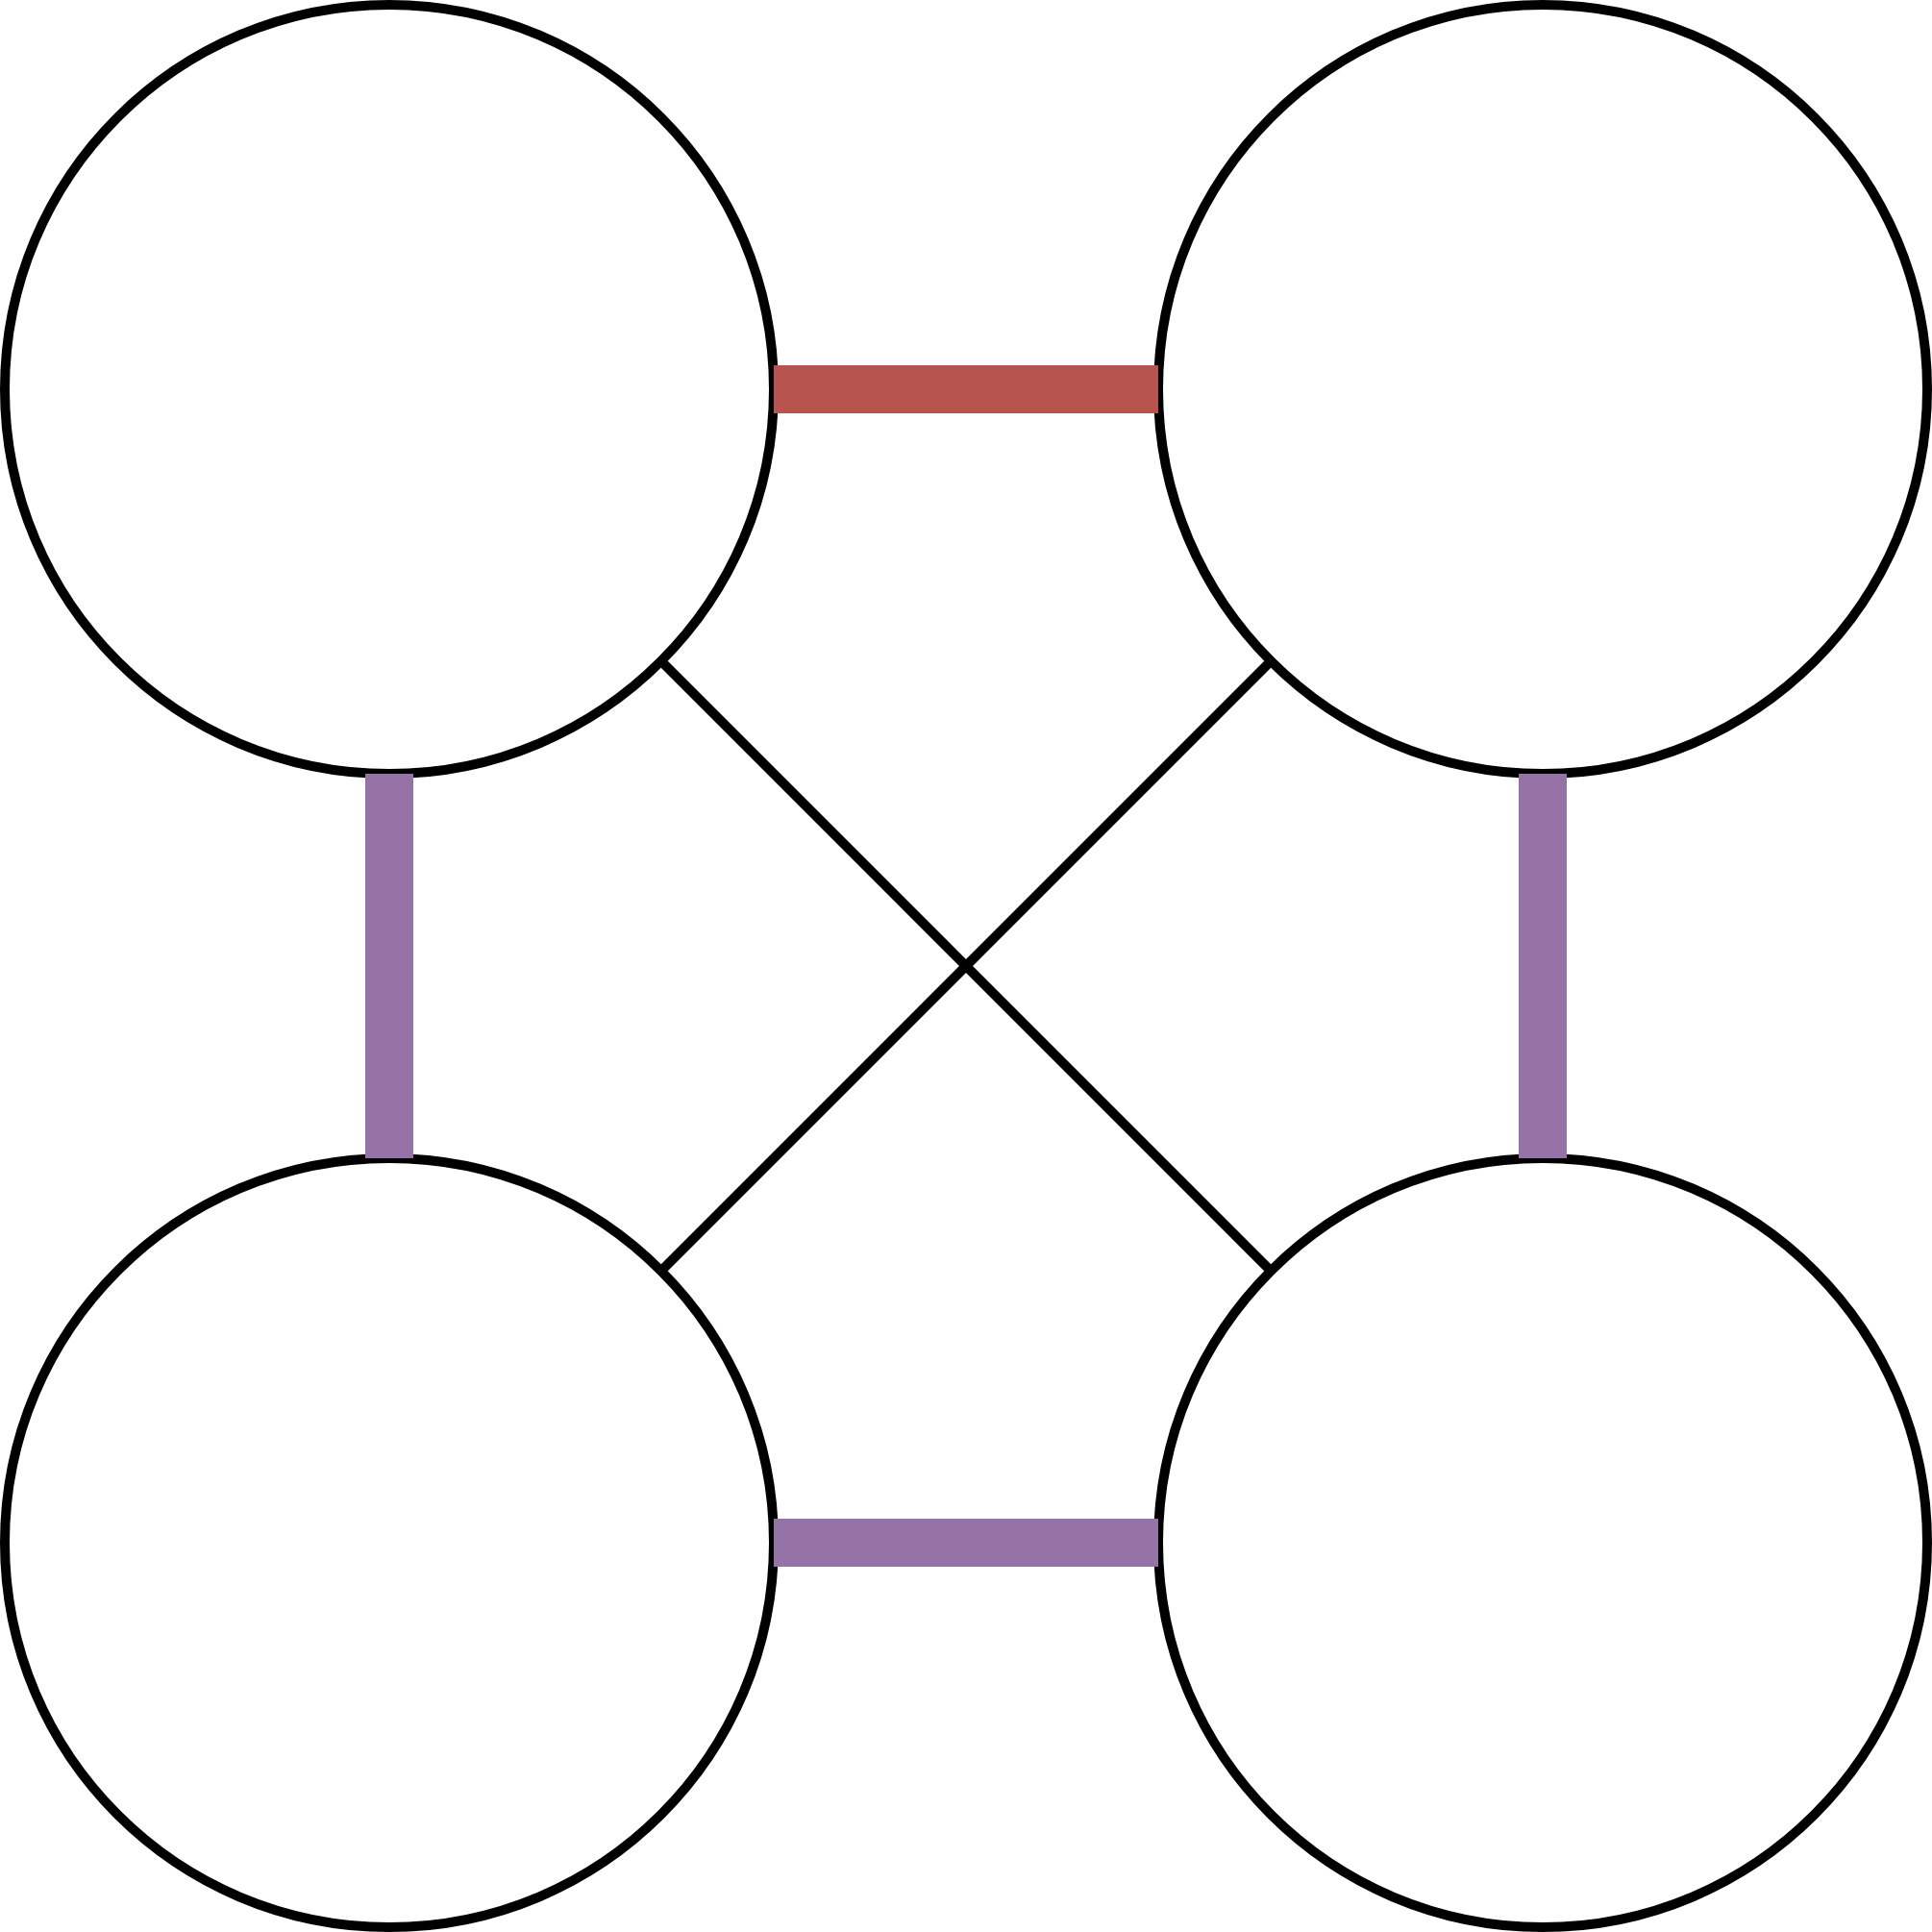
\includegraphics[height=2cm]{complete2.png}
\end{center}
\end{frame}

\subsection{MST vs.\ TSP tour}
\begin{frame}{MST vs.\ TSP tour}
\begin{center}
	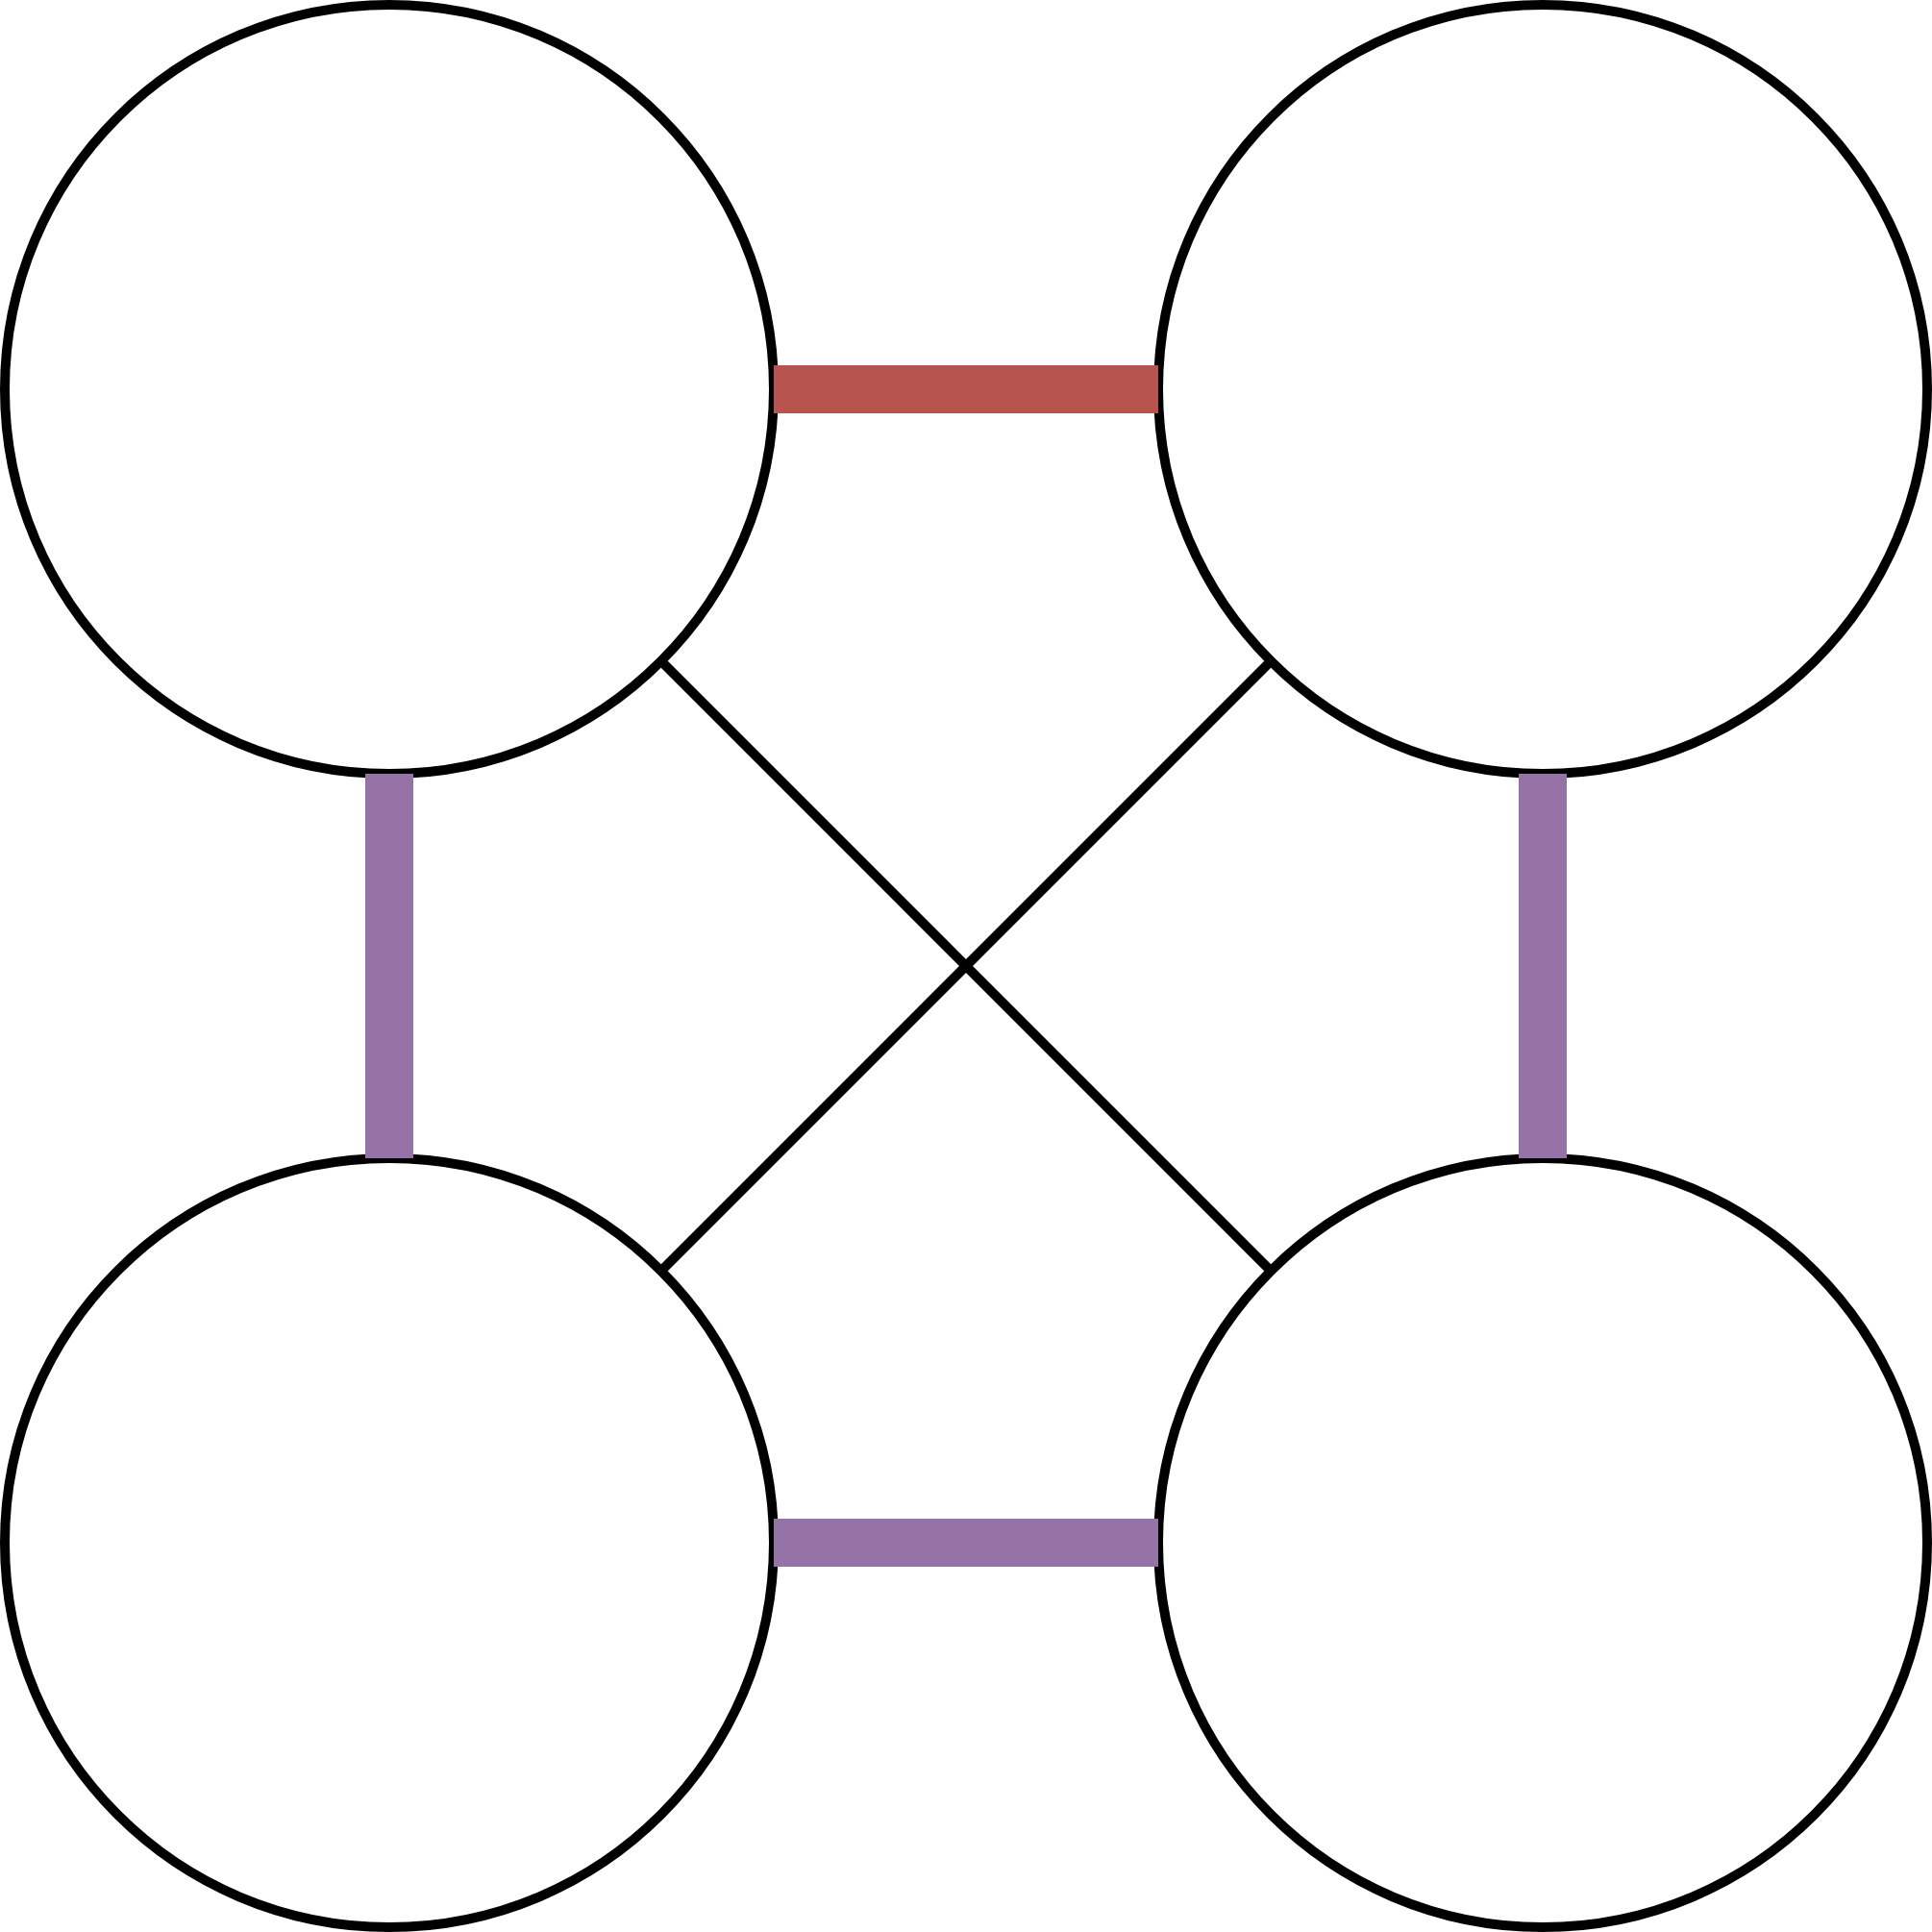
\includegraphics[height=2cm]{complete2.png}
\end{center}
\begin{isabelle}
\isacommand{lemma}\isamarkupfalse%
\ minimum{\isacharunderscore}spanning{\isacharunderscore}tree{\isacharunderscore}le{\isacharunderscore}OPTWEIGHT{\isacharcolon}\isanewline
\ \ \isakeyword{assumes}\ {\isacartoucheopen}minimum{\isacharunderscore}spanning{\isacharunderscore}tree\ T{\isacharprime}\ {\isacharparenleft}symhull\ E{\isacharparenright}{\isacartoucheclose}\isanewline
\ \ \isakeyword{assumes}\ {\isacartoucheopen}{\isadigit{2}}\ {\isasymle}\ card\ V{\isacartoucheclose}\isanewline
\ \ \isakeyword{shows}\ {\isacartoucheopen}set{\isacharunderscore}cost\ T{\isacharprime}\ {\isasymle}\ OPTWEIGHT{\isacartoucheclose}
\end{isabelle}
\end{frame}

\subsection{Tour Search}
\begin{frame}{Tour Search}
Find an edge sequence which\pause
\begin{itemize}
	\item uses exactly the MST's edges, each of which twice\pause
	\item visits every node\pause
	\item starts and ends at the same node\pause
\end{itemize}
This sequence is then called a \textit{pretour}.\pause

Its cost is twice the cost of the MST's edges.
%And the MST's edges are, as mentioned, less than the cost of an optimal tour.
\end{frame}

\subsection{Duplicate Removal}
\begin{frame}{Duplicate Removal}
Transform the pretour into a TSP tour:
%typically we require TSP tours to visits each node exactly once. Our sequence doesn't do that yet.
\begin{itemize}
	\item remove duplicate visits, replace them by shortcuts.\pause
	%That means that when the sequence goes to an already visited node, we instead jump to the next one
	
	\high{This can be done at one go.}
\end{itemize}
These shortcuts always exist and do not increase the cost. %That is why we require a complete metric graph
\end{frame}

\subsection{Time Complexity}%not verified
\begin{frame}{Time Complexity}\pause
\begin{itemize}
	\item MST generation: $\mathcal{O}(|E| \log |E|) = \mathcal{O}(n^2 \log (n^2)) = \mathcal{O}(2(n^2 \log n)) = \mathcal{O}(n^2 \log n)$%We use Kruskal's, which sorts edges by comparisons
	\pause
	\item Tour: $\mathcal{O}(n)$ %This is the number of edges in the MST. We discuss later how we can arrange the edges in time linear to this, to-do: Is this actually covered?
	\pause
\end{itemize}
overall: $\mathcal{O}(n^2 \log n)$
\end{frame}

\section{Results}
%What I did in the setting of this algorithm
\begin{frame}
\begin{center}
	\huge\high{Results}
\end{center}
\end{frame}

\subsection{Algorithm Sketch}
\begin{frame}{Algorithm Sketch} %and its Specification?
%We have a fixed graph here, OPT depends on it
\begin{isabelle}
	\isacommand{definition}\isamarkupfalse%
	\ two{\isacharunderscore}approx\ \isakeyword{where}\isanewline
	\ \ {\isacartoucheopen}two{\isacharunderscore}approx\ {\isacharequal}\ SPEC\ {\isacharparenleft}{\isasymlambda}T{\isachardot}\ is{\isacharunderscore}tour\ T\ {\isasymand}\ cost\ T\ {\isasymle}\ OPT\ {\isacharplus}\ OPT{\isacharparenright}{\isacartoucheclose}%explain lack of multiplication
	\vspace{1mm}\pause\\
	\isacommand{definition}\isamarkupfalse%
	\ algorithm{\isacharunderscore}sketch\ \isakeyword{where}\ {\isacartoucheopen}algorithm{\isacharunderscore}sketch\ {\isacharequal}\isanewline
	do\ {\isacharbraceleft}\isanewline
	\ \ MST\ {\isasymleftarrow}\ SPEC\ {\isacharparenleft}{\isasymlambda}E{\isacharprime}{\isachardot}\ minimum{\isacharunderscore}spanning{\isacharunderscore}tree\ {\isacharparenleft}ind\ E{\isacharprime}{\isacharparenright}\ G{\isacharparenright}{\isacharsemicolon}\isanewline
	\ \ pretour\ {\isasymleftarrow}\ SPEC\ {\isacharparenleft}{\isasymlambda}pT{\isachardot}\ int{\isacharunderscore}vertices\ pT\ {\isacharequal}\ nodes\ G\\ \ \ \ \ {\isasymand}\ cost\ pT\ {\isasymle}\ set{\isacharunderscore}cost\ MST\ {\isacharplus}\ set{\isacharunderscore}cost\ MST{\isacharparenright}{\isacharsemicolon}\isanewline
	\ \ tour\ {\isasymleftarrow}\ SPEC\ {\isacharparenleft}{\isasymlambda}T{\isachardot}\ is{\isacharunderscore}tour\ T\ {\isasymand}\ cost\ T\ {\isasymle}\ cost\ pretour{\isacharparenright}{\isacharsemicolon}\isanewline
	\ \ RETURN\ tour\isanewline
	{\isacharbraceright}{\isacartoucheclose}
\end{isabelle}\pause
\vspace{-4mm}
\begin{theorem}
	\hspace{2.6cm}$\textit{algorithm{\isacharunderscore}sketch} \le \textit{two{\isacharunderscore}approx}$\\
\upshape if $G$ is a complete finite metric graph.
\end{theorem}
\end{frame}

\subsection{Phase I}%MST generation
%It was already in a library, but had to be adjusted
\begin{frame}{Phase I}

\begin{isabelle}
	\isacommand{locale}\isamarkupfalse%
	\ finite{\isacharunderscore}weighted{\isacharunderscore}connected{\isacharunderscore}graph\ {\isacharequal}\ finite{\isacharunderscore}weighted{\isacharunderscore}graph\ {\isacharplus}\ connected{\isacharunderscore}graph\isanewline
	\isakeyword{begin}\isanewline
	\isanewline
	\ \ \isacommand{lemma}\isamarkupfalse%
	\ kruskal{\isadigit{0}}{\isacharunderscore}MST{\isacharcolon}\ {\isacartoucheopen}s{\isachardot}kruskal{\isadigit{0}}\ {\isasymle}\ SPEC\ {\isacharparenleft}{\isasymlambda}E{\isacharprime}{\isachardot}\ minimum{\isacharunderscore}spanning{\isacharunderscore}tree\ {\isacharparenleft}ind\ E{\isacharprime}{\isacharparenright}\ G{\isacharparenright}{\isacartoucheclose}
	\isanewline
	\isanewline
	\isacommand{end}\isamarkupfalse%
\end{isabelle}\pause%This also includes that the forest is a tree (simple) and that it still is minimal in the symhull (quite a bit of work...)

\begin{isabelle}
	\isacommand{sublocale}\isamarkupfalse%
	\ complete{\isacharunderscore}finite{\isacharunderscore}weighted{\isacharunderscore}graph\ {\isasymsubseteq}\\ \ \ finite{\isacharunderscore}weighted{\isacharunderscore}connected{\isacharunderscore}graph
	\end{isabelle}\pause
This required a reorganisation in the \textit{Kruskal} AFP entry.
\end{frame}

\subsection{Library Connections}
\begin{frame}{Library Connections}\pause
\vspace{3mm}
\begin{enumerate}
	\item \textit{Kruskal}: edges with weight field, undirected/directed\pause
	%to-do: vielleicht unterringeln?
	% I improved this library: I had to reorganise this one to get what I want without unnecessary assumptions.
	\item \textit{DFS\_Framework}: edges are node relations, directed\pause
	\item \textit{Koenigsberg\_Friendship}: edges have a label, undirected\pause
	%Even worse, there are different notions of "undirected"
	%So we really have the worst case in terms of compatibility.
	%Koenigsberg-Friendship also forbids loops, for technical reasons
	%It also reinterprets..., Kruskal also has a definition "is_path_undir".
	%to-do: add Noschinski, a third notion of "undirected".
	%"There are even more graph libraries out there: The somewhat new work by Noschinski starts anew,
	% with the reasonable modeling of undirected edges as two-element-sets (It sounds reasonable, and is well argued for).
	%Sadly, the fresh start did not really establish a new standard."
\end{enumerate}
%Example Conversion:\pause
\begin{isabelle}
\isacommand{lemma}\isamarkupfalse%
\ ex{\isadigit{1}}{\isacharunderscore}the{\isacharunderscore}path{\isacharcolon}\isanewline
\ \ \isakeyword{assumes}\ {\isacartoucheopen}is{\isacharunderscore}path{\isacharunderscore}undir\ G\ v\ ps\ v{\isacharprime}{\isacartoucheclose}\isanewline
\ \ \isakeyword{shows}\ {\isacartoucheopen}{\isasymexists}{\isacharbang}ps{\isacharprime}{\isachardot}\ map\ fst\ ps{\isacharprime}\ {\isacharequal}\ map\ fst\ ps\ {\isasymand}\ is{\isacharunderscore}path{\isacharunderscore}undir\ G\ v\ ps{\isacharprime}\ v{\isacharprime}{\isacartoucheclose}
\isanewline \pause
\isanewline
	\isacommand{definition}\isamarkupfalse%
	\ the{\isacharunderscore}path\ \isakeyword{where}\isanewline
	\ \ {\isacartoucheopen}the{\isacharunderscore}path\ nodelist\ lst\ {\isacharequal}\ {\isacharparenleft}case\ nodelist\ of\isanewline
	\ \ \ \ {\isacharbrackleft}{\isacharbrackright}\ {\isasymRightarrow}\ {\isacharbrackleft}{\isacharbrackright}\ {\isacharbar}\isanewline
	\ \ \ \ n\ {\isacharhash}\ ns\ {\isasymRightarrow}\ THE\ ps{\isachardot}\ map\ fst\ ps\ {\isacharequal}\ nodelist\\\ \ \ \ \ \ {\isasymand}\ is{\isacharunderscore}path{\isacharunderscore}undir\ G\ n\ ps\ lst{\isacharparenright}{\isacartoucheclose}
\end{isabelle}

\end{frame}

\subsection{Library Connections -- Example}
\begin{frame}{Library Connections -- Example}\pause
\begin{isabelle}
	\isacommand{lemma}\isamarkupfalse%
	\ spanning{\isacharunderscore}forest{\isacharunderscore}symhull{\isacharcolon}\isanewline
	\ \ {\isacartoucheopen}spanning{\isacharunderscore}forest\ F\ {\isasymlparr}nodes{\isacharequal}V{\isacharcomma}\ edges\ {\isacharequal}\ E{\isasymrparr}\ \\\ \ \ \ {\isasymLongrightarrow}\ spanning{\isacharunderscore}forest\ F\ {\isasymlparr}nodes{\isacharequal}V{\isacharcomma}\ edges\ {\isacharequal}\ symhull\ E{\isasymrparr}{\isacartoucheclose}
\end{isabelle}\pause
\begin{isabelle}
	\isacommand{lemma}\isamarkupfalse%
	\ {\isacharparenleft}\isakeyword{in}\ finite{\isacharunderscore}weighted{\isacharunderscore}graph{\isacharparenright}\\\ \ spanning{\isacharunderscore}forest{\isacharunderscore}symhull{\isacharunderscore}preimage{\isacharcolon}\isanewline
	\ \ \isakeyword{assumes}\ {\isacartoucheopen}spanning{\isacharunderscore}forest\ {\isasymlparr}nodes{\isacharequal}V{\isacharcomma}\ edges{\isacharequal}F{\isasymrparr}\ {\isasymlparr}nodes{\isacharequal}V{\isacharcomma}\\\ \ \ \  edges{\isacharequal}symhull\ E{\isasymrparr}{\isacartoucheclose}\isanewline
	\ \ \isakeyword{shows}\ {\isacartoucheopen}{\isasymexists}F{\isacharprime}{\isachardot}\\\ \ \ \ spanning{\isacharunderscore}forest\ {\isasymlparr}nodes{\isacharequal}V{\isacharcomma}\ edges{\isacharequal}F{\isacharprime}{\isasymrparr}\ {\isasymlparr}nodes{\isacharequal}V{\isacharcomma}\ edges{\isacharequal}E{\isasymrparr}\isanewline
	\ \ \ \ {\isasymand}\ edge{\isacharunderscore}weight\ {\isasymlparr}nodes{\isacharequal}V{\isacharcomma}\ edges{\isacharequal}F{\isacharprime}{\isasymrparr}\ \\\ \ \ \ \ \  {\isacharequal}\ edge{\isacharunderscore}weight\ {\isasymlparr}nodes{\isacharequal}V{\isacharcomma}\ edges{\isacharequal}F{\isasymrparr}{\isacartoucheclose}
\end{isabelle}
\end{frame}

\subsection{Phase II}
\begin{frame}{Phase II}
\begin{center}
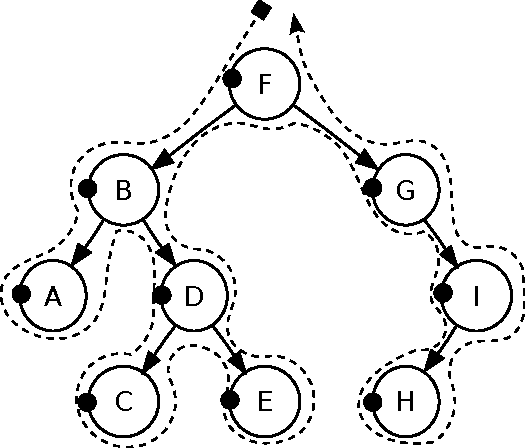
\includegraphics[height=7cm]{Sorted_binary_tree_preorder}
\end{center}
%to-do: attribute "By Sorted_binary_tree.svg: Milesderivative work: Pluke (talk) - Sorted_binary_tree.svg, Public Domain, https://commons.wikimedia.org/w/index.php?curid=10616003"
\end{frame}

\subsection{Phase II -- Parametrisation} %to-do: replace according to e-mail
\begin{frame}{Phase II -- Parametrisation}
\vspace{8mm}
We use the \textit{DFS-Framework}. This is the parametrisation:
\vspace{-2mm}
\begin{isabelle}
	\isacommand{definition}\isamarkupfalse%
	\ fp{\isadigit{0}}{\isacharunderscore}params\ {\isacharcolon}{\isacharcolon}\ {\isachardoublequoteopen}{\isacharprime}v\ fp{\isadigit{0}}{\isacharunderscore}param{\isachardoublequoteclose}\ \isakeyword{where}\isanewline
	{\isachardoublequoteopen}fp{\isadigit{0}}{\isacharunderscore}params\ {\isasymequiv}\ dflt{\isacharunderscore}parametrization\ state{\isachardot}more\isanewline
	\ \ {\isacharparenleft}RETURN\ {\isasymlparr}\ tour{\isacharunderscore}list\ {\isacharequal}\ {\isacharbrackleft}{\isacharbrackright}\ {\isasymrparr}{\isacharparenright}\isanewline
	\ \ {\isasymlparr}on{\isacharunderscore}discover\ {\isacharcolon}{\isacharequal}\ {\isasymlambda}{\isacharunderscore}\ n\ s{\isachardot}\ RETURN\ {\isasymlparr}tour{\isacharunderscore}list\ {\isacharequal}\ tour{\isacharunderscore}list\ s\ {\isacharat}\ {\isacharbrackleft}n{\isacharbrackright}{\isasymrparr}\ {\isasymrparr}{\isachardoublequoteclose}
\end{isabelle}\pause
\vspace{-5mm}
\begin{isabelle}
	\isacommand{locale}\isamarkupfalse%
	\ node{\isacharunderscore}and{\isacharunderscore}MST{\isacharunderscore}in{\isacharunderscore}graph\ {\isacharequal}\isanewline
	\ \ complete{\isacharunderscore}finite{\isacharunderscore}metric{\isacharunderscore}graph\ G\ {\isacharplus}\isanewline
	\ \ T{\isacharcolon}\ tree\ T\isanewline
	\ \ \isakeyword{for}\ G{\isacharcolon}{\isacharcolon}{\isacartoucheopen}{\isacharparenleft}{\isacharprime}v{\isacharcolon}{\isacharcolon}metric{\isacharunderscore}space{\isacharcomma}real{\isacharparenright}\ graph{\isacartoucheclose}\isanewline
	\ \ \isakeyword{and}\ T{\isacharcolon}{\isacharcolon}{\isacartoucheopen}{\isacharparenleft}{\isacharprime}v{\isacharcomma}real{\isacharparenright}\ graph{\isacartoucheclose}\ {\isacharplus}\isanewline
	\ \ \isakeyword{fixes}\ v\isactrlsub {\isadigit{0}}{\isacharcolon}{\isacharcolon}{\isacartoucheopen}{\isacharprime}v{\isacartoucheclose}\isanewline
	\ \ \isakeyword{assumes}\ v{\isacharunderscore}in{\isacharunderscore}V{\isacharcolon}\ {\isacartoucheopen}v\isactrlsub {\isadigit{0}}\ {\isasymin}\ V{\isacartoucheclose}\isanewline
	\ \ \isakeyword{and}\ mst{\isacharcolon}\ {\isacartoucheopen}minimum{\isacharunderscore}spanning{\isacharunderscore}tree\ T\ G{\isacartoucheclose}
\end{isabelle}
\end{frame}

%to-do: simplification of Phase II? not really my work, but something which slowed me down...

\section{Plans}
\begin{frame}
\begin{center}
	\huge\high{Plans}%time ran out sadly...
\end{center}
\end{frame}

\subsection{Input Generation}% We need a script that generates the edge weights for us.
\begin{frame}{Input Generation}
Consider a Euclidean space like $\RR^2$, $\RR^3$,\dots
	\begin{itemize}
		\item A popular metric is the \textit{Euclidean} metric.\pause
		
		\bad{It is often irrational, and thus difficult to store and compare with infinite precision.}\pause
		\item In contrast, the \textit{maximum metric} and the \textit{Manhattan metric} return natural numbers. %When the coordinates are natural numbers.
		%to-do: definition? small drawing?
	\end{itemize}
	%application drilling robot
\end{frame}

\subsection{DFS Invariant}
\begin{frame}{DFS Invariant}\pause
	finish this proof\pause
	\vspace{-2mm}
	\begin{isabelle}
		\isacommand{lemma}\isamarkupfalse%
		\ {\isacartoucheopen}dfs{\isachardot}is{\isacharunderscore}invar\ {\isacharparenleft}{\isasymlambda}s{\isachardot}\ valid{\isacharunderscore}graph{\isachardot}tour\ {\isacharparenleft}ind{\isacharprime}\ {\isacharparenleft}dom\ {\isacharparenleft}discovered\ s{\isacharparenright}{\isacharparenright}{\isacharparenright}\ {\isacharparenleft}tour{\isacharunderscore}list\ s{\isacharparenright}{\isacharparenright}{\isacartoucheclose}
	\end{isabelle}\pause
	Advancing this proof has already led to generally useful statements for the \textit{DFS-Framework}, e.g.\ \pause
	\begin{isabelle}
		\isacommand{lemma}\isamarkupfalse%
		\ i{\isacharunderscore}snd{\isacharunderscore}pending{\isacharunderscore}sane{\isacharcolon}\ {\isacartoucheopen}dfs{\isachardot}is{\isacharunderscore}invar\ {\isacharparenleft}{\isasymlambda}s{\isachardot}\ snd\ {\isacharbackquote}\ {\isacharparenleft}pending\ s{\isacharparenright}\ {\isasymsubseteq}\ V{\isacharparenright}{\isacartoucheclose}
	\end{isabelle}\pause
	\begin{isabelle}
		\isacommand{lemma}\isamarkupfalse%
		\ i{\isacharunderscore}stack{\isacharunderscore}sane{\isacharcolon}\ {\isacartoucheopen}dfs{\isachardot}is{\isacharunderscore}invar\ {\isacharparenleft}{\isasymlambda}s{\isachardot}\ set\ {\isacharparenleft}stack\ s{\isacharparenright}\ {\isasymsubseteq}\ V{\isacharparenright}{\isacartoucheclose}
	\end{isabelle}\pause
	\begin{isabelle}
		\isacommand{lemma}\isamarkupfalse%
		\ i{\isacharunderscore}discovered{\isacharunderscore}sane{\isacharcolon}\ {\isacartoucheopen}dfs{\isachardot}is{\isacharunderscore}invar\ {\isacharparenleft}{\isasymlambda}s{\isachardot}\ dom\ {\isacharparenleft}discovered\ s{\isacharparenright}\ {\isasymsubseteq}\ V{\isacharparenright}{\isacartoucheclose}
	\end{isabelle}
\end{frame}

\section{Conclusion}
\begin{frame}{Conclusion}
Even with parts already verified, formal verification can require a lot of work:
\begin{itemize}
	\item Differing graph formalisations\pause!\pause
	%in particular connecting Digraph.graph_rec to my own finite_complete_weighted...graph
	\item For this particular algorithm, a lot of assumptions have to be collected and formulated.\pause %complete_finite_weighted is actually complete_finite_weighted_simple_loopfree_metric_graph
	
	%"Not really part of a conclusion, but I want to mention it here since I had to leave out much context earlier for brevity."
	\item Definitions have many dependencies. %They e.g. have to fix a graph, a subtree and an arbitrary node at the same time.
\end{itemize}
\end{frame}

\section{Questions}
\begin{frame}
\begin{center}
	\huge\high{Questions}
\end{center}
\end{frame}

%to-do: Problems?

\end{document}

%to-do: compare to the plan from the meeting:
%25+5min

%explain in the presentation:

%Bibliotheken vorstellen, Wahl begründen
%--> Graphformalisierungen: directed vs. undirected edges in both phases. Welche gibt es alle?
%edge labels, i.e. a third field besides start node and end node 5min
%MST lemma zeigen, wieso nicht Graph_Theory? 5min
%was ist der projektstatus? 5min
%maybe a slide about the commit count?
%add dfs-sublocale statement to plans. "This is already proven. However, the set membership must be implemented..."
